\documentclass[12pt,fleqn]{article}\usepackage{../../common}
\begin{document}
Ders 10

Lineer cebirin özüne iniyoruz şimdi, 4 temel altuzay nedir ve onların
arasındaki ilişki nasıldır? 

Dört Temel Altuzay

1) Kolon uzayı $C(A)$ (columnspace). Boyutları $m \times n$ olan $A$
matrisinin her kolonunun $m$ tane öğesi / hücresi vardır, o zaman $C(A)$
uzayı $\mathbb{R}^m$ içindedir.

2) Sıfır uzayı, $N(A)$ (nullspace)

3) Satır uzayı (rowspace), bir matrisin satırlarının tüm kombinasyonu. Bu kombinasyon
hakkında başka hangi kelimeyi kullanabilirim? Satırlar satır uzayını kapsar
(span). $A$'nin satırları bu uzay için bir baz (basis) oluşturur mu? Belki
evet, belki hayır. Eğer satırlar birbirinden bağımsız ise evet. 

Akla gelen bir fikir şu olabilir, satırlar ile uğraşmayı sevmiyorum,
şimdiye kadar kolonlar üzerinden işleyen bir sürü araç / dil geliştirdik,
bunları kullanmaya devam etmek istiyorum. O zaman basit bir çözüm şu,
$A$'nin devriğini alırım, böylece satırlar kolon haline gelir ve ben de
$A^T$'nin kolonlarıyla iş yapmaya devam ederim. Bildik notasyonu
kullanabilirim, $C(A^T)$ mesela. Bunun işleyip işlemediğini göreceğiz.

4) $A^T$'nin sıfır uzayı, $N(A^T)$. Bu sıfır uzayına ``$A$'nin sol sıfır
uzayı'' adı da veriliyor.

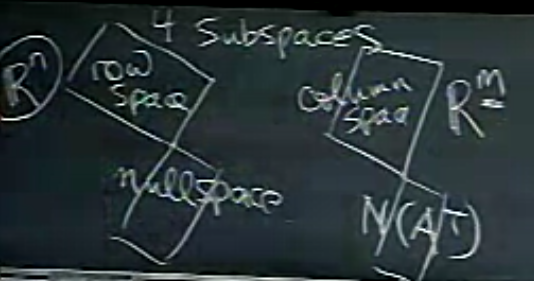
\includegraphics[height=4cm]{10_01.png}

Temel altuzaylar hakkında bilmek istediklerim şunlar: Bu uzayların bazı
nedir? Boyutları nedir? 

$C(A)$'nin boyutu $A$'nin kertesi $r$. Bunu önceki derste bir örnek
üzerinden görmüştük. 

Satır uzayının, yani $C(A^T)$'nin boyutu aynen $C(A)$ gibi $r$'ye eşit, yani
matris kertesi ile aynı.

Alttaki matrisin satır boyutu nedir? 

$$ 
\left[\begin{array}{rrr}
1 & 2 & 3 \\
1 & 2 & 3 \\
2 & 5 & 8 
\end{array}\right]
 $$

Boyut sayısı 2'dır. Satırlara bakınca 1. ve 2. satır aynı, bağımsız sadece iki
tane satır var. Kolon ve satır uzaylarının boyut eşitliği kuralından
hareketle, o zaman kolon uzayı boyutu da 2. Eliminasyon sırasında 2 tane
pivot kolonu çıkacaktır, ve kolonlar da bağımlıdır. Bu örnek aslında
ilginç çünkü kolonlara bakınca bağımlılık bariz değil (3. kolon 1. ve
2. kolonun direk toplamı değil mesela), ama satırlara bakınca bağımlılık
belli oluyor.
 
Sıfır uzayı için baz özel çözümlerdir, ki eğer hatırlarsak, her serbest
değişken için bir özel çözüm vardır. Özel çözüm sayısı ise $n-r$, o zaman
sıfır uzayı boyutu $n-r$. Demek ki sıfır uzay için özel çözümler bir baz
oluştururlar. 

$N(A^T)$'nin boyutu ise $m-r$, çünkü $A^T$'nin kolon sayısı $A$'nin satır
sayısı, kolon sayısını elde edince geri kalan işlem üstteki sıfır uzayı ile
aynı, $N(A^T)$'nin serbest değişken sayısı devreye girer, vs. 

Şimdi baz bulma konusuna dönelim; kolon uzayının bazını bulmayı biliyoruz,
pivot içeren kolonlar baz oluşturur. Peki satır uzayı için bazı nasıl
buluruz? Akla hemen şu gelebilir, matrisin devriğini alırım, ve o devrik
üzerinde bildiğim işlemleri yaparım, eliminasyon, pivot bulma, vs. Ama bu
fikre balıklama atlamadan önce, acaba bildiğimiz tekniği olduğu gibi
kullanmak acaba daha iyi bir fikir olabilir mi? Bir örneğe bakalım, klasik
eliminasyon senaryosu uygulayalım,

$$ 
\left[\begin{array}{rrrr}
1 & 2 & 3 & 1 \\
1 & 1 & 2 & 1 \\
1 & 2 & 3 & 1
\end{array}\right] \rightarrow
\left[\begin{array}{rrrr}
1 & 2 & 3 & 1 \\
0 & -1 & -1 & 0 \\
0 & 0 & 0 & 0
\end{array}\right]
 $$

İkinci pivot'ta eksi olmayan değer istiyorum, 2. satırı -1 ile
çarpayım. Sonra 2. satır 2 ile çarpıp 1. satırdan çıkartayım,

$$ R =
\left[\begin{array}{rrrr}
1 & 0 & 1 & 1 \\
0 & 1 & 1 & 0 \\
0 & 0 & 0 & 0
\end{array}\right]
 $$

Bunlar bildiğimiz işlemler. Şimdi sol üst köşede $2 \times 2$ boyutlu $I$ var,
hemen yanında $F$, ve en alt satır sıfır.

Neler olduğuna dikkat edelim, üstteki işlemler sırasında matrisin kolon
uzayı değişti. Yani artık $A$'nin kolon uzayı $R$'nin kolon uzayı ile aynı
değil, $C(A) \ne C(R)$. Satır işlemleri yaptık (satır uzayı değişmedi), ve
kolon uzayında değişime sebep olduk. 

Neyse; şimdi $R$'nin satır uzayı için baz nedir, ki bu baz $A$'nin aynı
olan satır uzayı için de aynı olacaktır? $R$'den bariz görülüyor, ilk iki
satırı, yani ilk $r$ satırı, baz oluşturur. Bu şekilde satır uzayını bulmak
faydalı çünkü eliminasyon sırasında $R$'yi zaten olabileceği en temiz hale
getiriyorum, bu işlem tamamlandıktan sonra $R$'den bazları çekip
çıkartabilirim. 

Bir soru: madem bir baz elde ettim, $A$'nin satırlarının $R$ satırlarının
kombinasyonu olup olmadığından nasıl emin olabilirim? Çok basit,
eliminasyon sırasında yaptığım işlemleri tersine çevirirsem, bir tür
kombinasyon işlemi yapmış olurum, ve bu kombinasyon bana kesinlikle $A$'nin
satırlarını verecektir, çünkü başlangıç noktam zaten $A$ idi. 

Nihayet son uzayımız, $N(A^T)$'nin uzayı için bir baz nasıl bulurum?

Bu uzaya niçin ``sol'' sıfır uzayı deniyor? 

Bu uzayın içinde vektörler vardır, tabii ki, $A^Ty = 0$ denklemini tatmin
eden $y$'ler bu vektörlerdir. Bu denklemin devriğini alırsam,

$$ y^TA = 0 $$

Bu denkleme göre yatay vektör $y^T$, $A$'yi ``soldan'' çarpıyor, 
sol sıfır uzayı sözü buradan geliyor. Fakat bu bir kullanım şekli tabii,
ben şahsen $A^Ty=0$ formunu tercih ediyorum [herhalde devrik alma sebebi
$A^T$'yi $A$ haline getirmek, bu işlem sırasında $y$ de ``sola'' geçmiş
oluyor]. 

Bazı nasıl bulurum? 

$A$ üzerinde pivot bulma, eliminasyon gibi işlemler bize $R$'yi vermişti,
bu işlemler tabii $A$ üzerindedir, $A^T$ üzerinde değildir, ama sezgisel
olarak bu işlemlerin bize sol sıfır uzayı hakkında da birşeyler söylediğini
tahmin edebiliriz. $A$'dan $R$'ye gelirken bazı işlemler yaptık, ve bu
işlemlerin tamamı ile ilgileniyorum, yani bu tüm işlemleri temsil eden o
tek matrisle ilgileniyorum. Bu matrisi nasıl buluruz? 

Gauss-Jordan'ı hatırlıyor musunuz? Hani matris üzerinde işlemler yaparken
ona yandan bir ekstra birim matrisi eklemiştik. GJ kullanımını bir kare
matrisin tersini almak için kullanmıştık. Şimdi matris kare değil,
çoğunlukla dikdörtgen, ama yine de birim matrisi ekleyebiliriz, 

$$ 
\left[\begin{array}{rr}
A_{m \times n} & I_{m \times m}
\end{array}\right]
 $$

Ve bu matris üzerinde rref uygularım. Sonuç ne olur? $A$ tabii ki $R$'ye
dönüşecek, aynı işlemler $I$ üzerinde de uygulanmış olacak, ve orada da
ortaya bir matris çıkacak, bu matrise $E$ matrisi diyelim,

$$ 
\left[\begin{array}{rr}
R_{m \times n} & E_{m \times m}
\end{array}\right]
 $$

Eğer düşünürsek $E$ matrisinin $A$ üzerinde yaptığımız tüm işlemlerin bir
kayıdı olduğunu görebiliriz. İşlemlerimizin arkada bıraktığı ``iz'' bu
$E$ içinde bir bakıma. O zaman şunu da söyleyebiliriz, $A$ üzerinde
yaptığımız işlemler $E$ içindeyse, o zaman 

$$ 
E
\left[\begin{array}{rr}
A_{m \times n} & I_{m \times m}
\end{array}\right] = 
\left[\begin{array}{rr}
EA & EI
\end{array}\right] = 
\left[\begin{array}{rr}
R_{m \times n} & E_{m \times m}
\end{array}\right]
 $$

çünkü 

$$ EA = R $$

Daha önce Gauss-Jordan gördüğümüzde amacımız matris tersi almaktı,
hedefimiz $R$'e erişmek değil, $I$'ya erişmekti, ve $E$ bize $A$'yi
değiştirip $A^{-1}$'yi vermişti. Burada hedef farklı, fakat ana fikir aynı.

Biraz önceki örneğimiz üzerinde görelim, 

$$ 
A = \left[\begin{array}{rrrr}
1 & 2 & 3 & 1 \\
1 & 1 & 2 & 1 \\
1 & 2 & 3 & 1
\end{array}\right]
 $$

Bu matrisi $R$'ye dönüştürmek için yaptığım tüm işlemleri $3 \times 3$
boyutlu bir $I$ üzerinde uygularsam, 

$$ 
\left[\begin{array}{rrr}
-1 & 2 & 0 \\
1 & -1 & 0 \\
-1 & 0 & 1 
\end{array}\right]
 $$

Bu zannediyorum ki $E$. Kontrol etmek için $A$'yi bu matrisle soldan
çarpalım, ve $R$'yi elde edip etmeyeceğimizi görelim,

$$ 
\left[\begin{array}{rrr}
-1 &  2 & 0 \\
1 & -1 & 0 \\
-1 & 0 & 1
\end{array}\right]
\left[\begin{array}{rrrr}
1 & 2 & 3 & 1 \\
1 & 1 & 2 & 1 \\
1 & 2 & 3 & 1
\end{array}\right]
 $$

\begin{minted}[fontsize=\footnotesize]{python}
E = np.array([[-1,2,0],[1,-1,0],[-1,0,1]])
A = np.array([[1,2,3,1],[1,1,2,1],[1,2,3,1]])
print np.dot(E,A)
\end{minted}

\begin{verbatim}
[[1 0 1 1]
 [0 1 1 0]
 [0 0 0 0]]
\end{verbatim}

Evet, $R$'yi elde ettik. 

Tüm bunları $A$'nin sol sıfır uzayını elde etmek için yaptım. Daha
ilerlemeden, bu arada, sol sıfır uzayının boyutu nedir? Boyut $m-r$, yani
3-2=1, yani boyut 1. Yani baz tek bir vektör, yani $A$'nin satırlarını
kombine edip sıfır sonucunu ortaya çıkarabilecek tek bir vektör var. 

O vektör nedir? $E$'nin son satırı bize o vektörü gösteriyor, çünkü o satır
$A$'yi soldan çarparken $A$'nin satırlarını kombine ederek $R$'nin tamamen
sıfır olan o son satırını ortaya çıkartmıştır. 

$$ R =
\left[\begin{array}{rrrr}
1 & 0 & 1 & 1 \\
0 & 1 & 1 & 0 \\
0 & 0 & 0 & 0
\end{array}\right]
 $$

Yani $R$'nin son satırına tekabül eden $E$'nin son satırı aradığımız
vektördür.

Bu sonucu bulmak için $E$'yi ortaya çıkartmamız gerekti, fakat bu işlem
daha doğal, $A$'nin devriğini alıp onun üzerinde daha çetrefil işlemler
yapmak gerekmedi. 

Dört altuzay işte bunlardır. 

Bu dersi kapatmadan önce şimdiye kadar görmediğimiz yeni bir tür vektör
uzayından bahsetmek istiyorum. 

Bir örnek, tüm $3 \times 3$ boyutundaki matrisler. Ama bir dakika
diyebilirsiniz, vs. boyutundaki matrisler nasıl bir {\em vektör} uzayı
ortaya çıkarabilirler. Fakat biraz düşünürsek, matrislerin vektör uzayı
oluşturmak için vektörler üzerinde uyguladığımız kurallara aynen
uyabileceğini görürüz. Matrislerin lineer kombinasyonlarını alabilirim,
onları bir skalar (tek sayı) ile çarpabilirim, vs. Vektör uzayları için
geçerli tüm kurallar burada da geçerli olabilir. 

Peki altuzaylara ne olur? Bu ``matris uzayının'', ki üstteki örnekteki
uzaya $M$ diyelim şimdilik, bir altuzayı var mıdır? Bir tane bulayım
mesela.. tüm $3 \times 3$ boyutundaki.. üstüçgensel matrisler. Ya da..
simetrik matrisler. Devam edelim; İki altuzayın kesişiminin yeni bir
altuzay olduğunu biliyoruz, hatta önceki bir derste bunu ispatlamıştık
bile, o zaman simetrik ve üstüçgensel matrislerin uzaylarının kesişimini
kullanabilir miyiz? İlginç bir durum bu aslında, çünkü üstüçgensel
matrislerin köşegeni (diagonal) altında tamamen sıfır vardır, eğer
simetriklik şartı arıyorsak, o zaman köşegenin üstü de sıfır olmalıdır, o
zaman geriye sadece köşegeninde değerler olan matrisler kalır, ki bu
matrisler köşegen (diagonal) matrislerdir. Bir altuzay da bu yani, köşegen
matrisler, tabii üstüçgensel ve simetrik matrislerin altuzayından daha
küçük bir altuzay. 

Bu kelimeyi kullanabilir miyim? Küçük? Bu durumda küçüklük ne demektir? Eh,
köşegen matrislerin altuzayı diğerlerinin içindedir, vs. Fakat daha
spesifik olarak altuzay boyutu kavramını kullanabilirim şimdi; Tabii boyut
için bir baz hesaplamam gerekli, bunu yapınca bu bazda kaç tane eleman
olduğunu sayarım ve sonucu bulurum. Köşegen matris altuzayı için, bence bu
sayı 3. Nereden biliyorum? Mesela üç tane matris yazacağım, 

$$ 
\left[\begin{array}{rrr}
1 & 0 & 0 \\
0 & 0 & 0 \\
0 & 0 & 0 
\end{array}\right], 
\left[\begin{array}{rrr}
1 & 0 & 0 \\
0 & 3 & 0 \\
0 & 0 & 0 
\end{array}\right], 
\left[\begin{array}{rrr}
0 & 0 & 0 \\
0 & 0 & 0 \\
0 & 0 & 7 
\end{array}\right]
 $$

Bence bu bir baz. Birbirinden bağımsızlar, ve tüm köşegen matrisler bu
üçünün bir kombinasyonu, yani bu üç matris tüm köşegen matrisler altuzayını
kapsıyorlar. 

Şimdiye kadar gördüğümüz fikirleri yeni bir ortam için bayağı esnettik,
fakat fikirler burada da geçerli. 

\end{document}
